\section{Background and Related Work}
\label{sec:relwork}
There is a related paper \cite{Ma23} that analyzes a model known as a recommendation system. In their work, they build the PyTEI package for injecting models. However, recommendation models differ significantly from LLMs so the overall effect could be quite different for the same error injections.

However, the paper does not do any evaluation on the different of hardware errors in specific parts of the recommendation system, so the question of whether particular parts are more vulnerable is still open.

An interesting part of this paper is the evaluation of possible mitigations against hardware flips, which can also be evaluated in the context of LLMs. In addition, their evaluation had limited scope, and it could be interesting to expand on their analysis by testing a wider variety of errors and examining the tradeoffs of each.

\cite{fidelity} performed resilience analysis on transient errors in logic components, but their framework is highly inefficient in the context of PyTorch, because they employ frequent to-and-back type conversions as PyTorch doesn't natively support bit operations in float tensors. \cite{thales} estimated DNN accuracy under transient faults and proposed a Monte Carlo-based estimation method. However, their analysis is also limited to transient errors and do not consider logic / data path errors which are permanent and more impactful.


\section{Threat model.}
An attacker's goal is to cause information disclosure or cause a denial of service via system crash or significantly degrading the performance of the LLM. They may attack components such as edge AI chips and accelerators, CPUs and GPUs in LLM training, memory systems storing model weights, and data transfer channels between hardware components. To induce hardware errors, they could somehow achieve write access to memory systems, or physical access to create fault-heavy environments (e.g. radiation source). 

\subsection{Case Studies}
We present 2 case studies, relating to information disclosure and denial of service respectively. However, for the purposes of this paper, we will investigate the effects of the \textit{denial of service} attack objective, specifically performance degradation only.

\subsubsection{Case 1 (Information Disclosure)} An LLM is running on an edge device (like a smartwatch). The attacker jailbreaks the device, gaining write access to hardware, and inject bit errors with a probability $p$. The attacker then monitors the LLM output through API calls, observing that the output is NaN XX\% of the time. The attacker thus concludes that the LLM has YY number of parameters (see \ref{sec:nan} for more details).

\subsubsection{Case 2 (Denial of Service)} A physics research lab is using LLMs for running simulations of their experiments. An attacker somehow manages to convince the lab scientists to house the servers the LLM is running on in their reactor chamber, a source with high radiation. This environment causes many bit flip errors, causing frequent faulty outputs from the LLM.

\begin{figure}[!htbp]
    \centering
    \begin{subfigure}[b]{\linewidth}
        \centering
        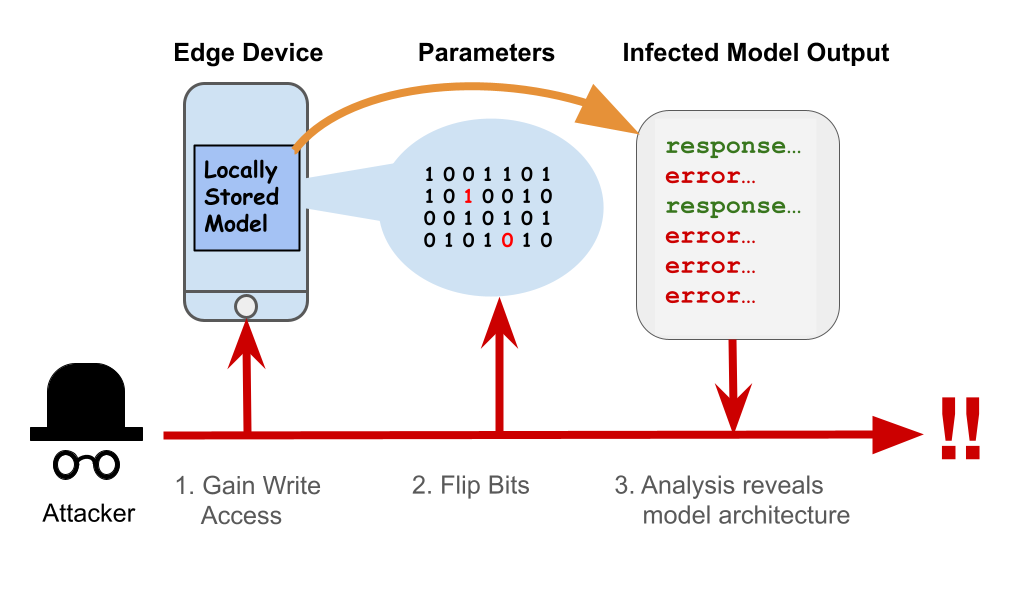
\includegraphics[width=1.0\linewidth]{images/threat-case-1.png}
    \end{subfigure}
    \vspace{1cm}
    \begin{subfigure}[b]{\linewidth}
        \centering
        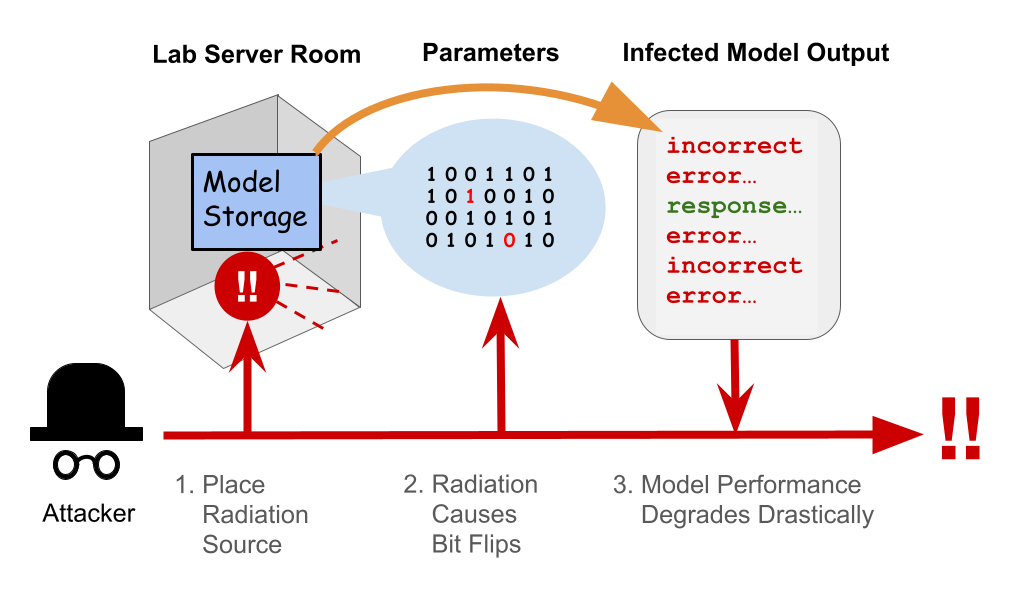
\includegraphics[width=1.0\linewidth]{images/threat-case-2.png}
    \end{subfigure}
    \caption{Threat models for case studies: Information Disclosure (top) and Denial of Service (bottom)}
    \label{fig:threatcases}
\end{figure}

\section{Overview of the design}
\label{sec:overview}

We chose Hugging Face's implementations of Mistral-7B \cite{jiang2023mistral7b} as our model of choice. We evaluated our models on \cite{hendrycks2021measuringmassivemultitasklanguage}, an open-source LLM benchmark, specifically the computer science and astronomy tests that have the injected LLM answer multiple choice questions. For each model with varying error rates, the score is computed as the proportions of correct answers.

\subsection{Design Choices}
We originally chose GPT2 but noticed a lot of NaN outputs. See \ref{sec:nan} for analysis. Hence, we switched to an error model that injects \textit{value} errors instead. \\

We also observed that GPT2 performance on the MMLU benchmark was equivalent to random guessing, which would not be informative of performance drops. We upgraded to Mistral-7B which has a 0.58 average accuracy.

\subsection{Design Approaches}
\subsubsection{Sequential Injection} 
To analyze the impact of errors in sequential layers on model accuracy, we grouped the decoder layers into sets of four. This grouping reduced computational overhead while still enabling the modeling of sequential error injection behavior. Weights within each group were tracked, and errors were injected with varying probabilities ranging from $10^-9$ to $10^-1$. For each error likelihood, the model’s accuracy on the MMLU benchmark was recorded.

\subsubsection{Functional Injection} 
In order to determine if, and what, components of an LLM (i.e Attention Mechanism, Embedding, etc) were less resistant to SDC, we chose to inject errors into weights associated with these components. For each component's weights, errors were injected with a varying probability from $10^{-9}$ to $10^{-1}$. For each likelihood of errors, model accuracy on the MMLU benchmark was recorded.

\begin{figure}[!htbp]
    \centering
    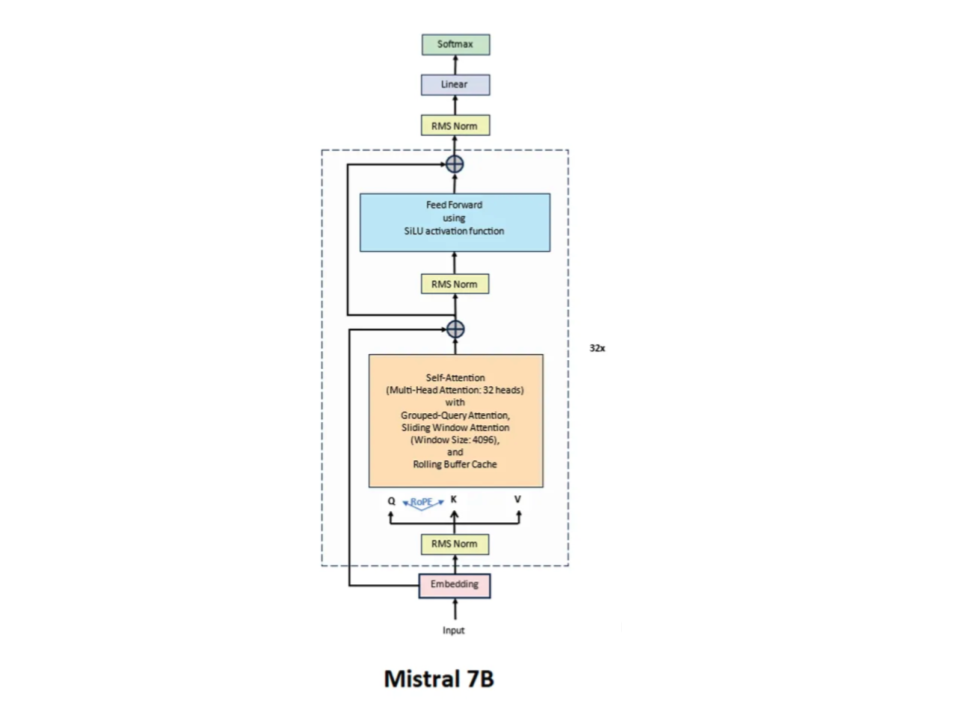
\includegraphics[width=1\linewidth]{images/Mistral-7B-Arch.png}
    \caption{Injected Model's Architecture}
    \label{fig:enter-label}
\end{figure}